In this section, results are presented for the
source-void-to-absorber test problem. This is a 1-D test problem
with zero incoming flux incident on the left boundary,
a constant source in a void in the left half of the
domain, and an absorber with no source in the right half of the
domain. The test problem description is given by Table
\ref{tab:source_void_to_absorber}.

%-------------------------------------------------------------------------------
\begin{table}[htb]\caption{Source Void-to-Absorber Test Problem Summary}
\label{tab:source_void_to_absorber}
\centering
\begin{tabular}{l l}\toprule
\emph{Parameter} & \emph{Value}\\\midrule
Domain & $\domain = (0,1)$\\
Initial Conditions & $u_0(x)=0$\\
Boundary Conditions & $u(0,t)=0 \eqc \quad t>0$\\
Direction & $\di = \mathbf{e}_x$\\
Cross Section & $\sigma(x)=\left\{\begin{array}{c l}
   0,  & x < \frac{1}{2}\\
   10, & \mbox{otherwise}\end{array}\right.$\\
Source & $q(\x,t)=\left\{\begin{array}{c l}
   1,  & x < \frac{1}{2}\\
   0,  & \mbox{otherwise}\end{array}\right.$\\
Speed & $\speed=1$\\
Exact Solution & $u(x,t)=\left\{\begin{array}{l l}
   \scalarsolution_{\text{ss}}(x), & x-t<0\\
   0, & \mbox{otherwise}
   \end{array}\right.$ \\
   & $\scalarsolution_{\text{ss}}(x) =
       \left\{\begin{array}{l l}
          e^{-10(x-\frac{1}{2})}, & x\ge\frac{1}{2}\\
          1,                      & \mbox{otherwise}
       \end{array}\right.$\\
\bottomrule\end{tabular}
\end{table}
%-------------------------------------------------------------------------------

Figure \ref{fig:source_void_to_absorber}
shows the results for this problem using SSPRK time discretization,
a CFL of 0.5, and 32 cells.
Entropy residual and jump coefficients $\entropyresidualcoef$ and
$\entropyjumpcoef$ are both 1.
Figure \ref{fig:source_void_to_absorber_fine} shows results
for a finer mesh (256 cells) that illustrates the shortcomings of Galerkin-FCT
vs. EV-FCT: Galerkin-FCT does not necessarily converge to the
entropy solution.

%%-------------------------------------------------------------------------------
%\begin{table}[ht]\caption{Source-Void-to-Absorber Test Problem Run Parameters}
%\label{tab:source_void_to_absorber_run_parameters}
%\centering
%\begin{tabular}{l l}\toprule
%\emph{Parameter} & \emph{Value}\\\midrule
%Number of Cells & $N_{cell} = 2^5, 2^8$\\
%End Time & $t = 1$\\
%CFL Number & $\nu = 0.5$\\
%Time Integrator & SSPRK33\\\midrule
%Entropy Function & $E(u) = \frac{1}{2}u^2$\\
%Entropy Residual Coefficient & $c_E = 1.0$\\
%Entropy Jump Coefficient & $c_J = 1.0$\\
%Entropy Time Integrator & BE\\
%\bottomrule\end{tabular}
%\end{table}
%-------------------------------------------------------------------------------
\begin{figure}[ht]
   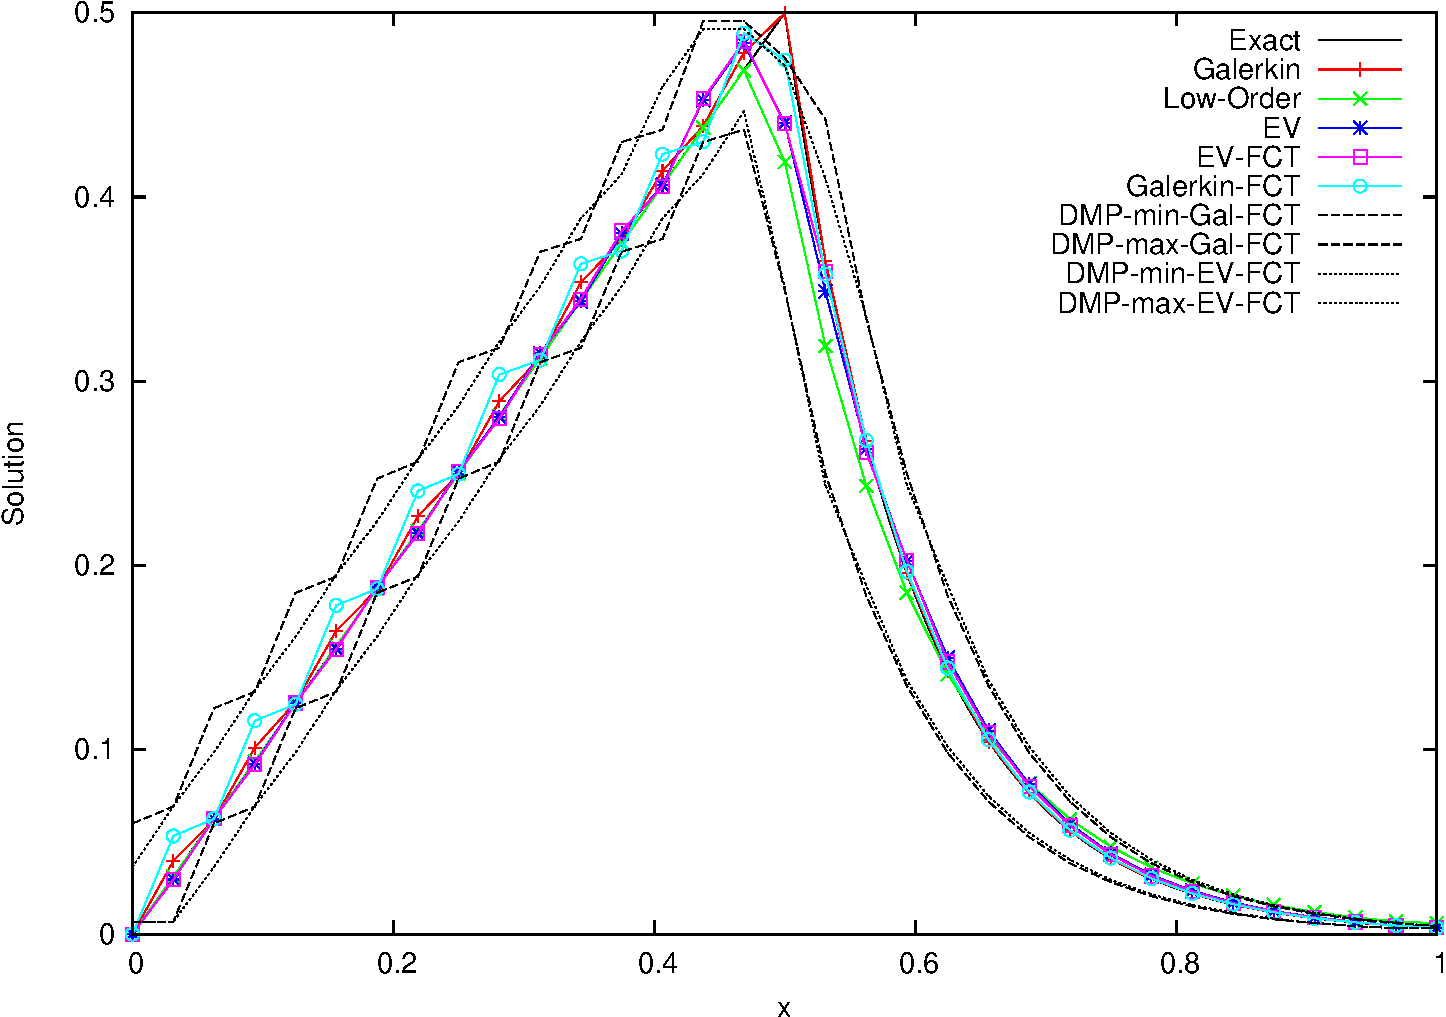
\includegraphics[width=\textwidth]
     {\contentdir/results/transport/source_void_to_absorber/coarse.pdf}
   \caption{Comparison of Solutions for Source-Void-to-Absorber Problem
     with $2^5$ Cells}
   \label{fig:source_void_to_absorber}
\end{figure}
%-------------------------------------------------------------------------------
\begin{figure}[ht]
   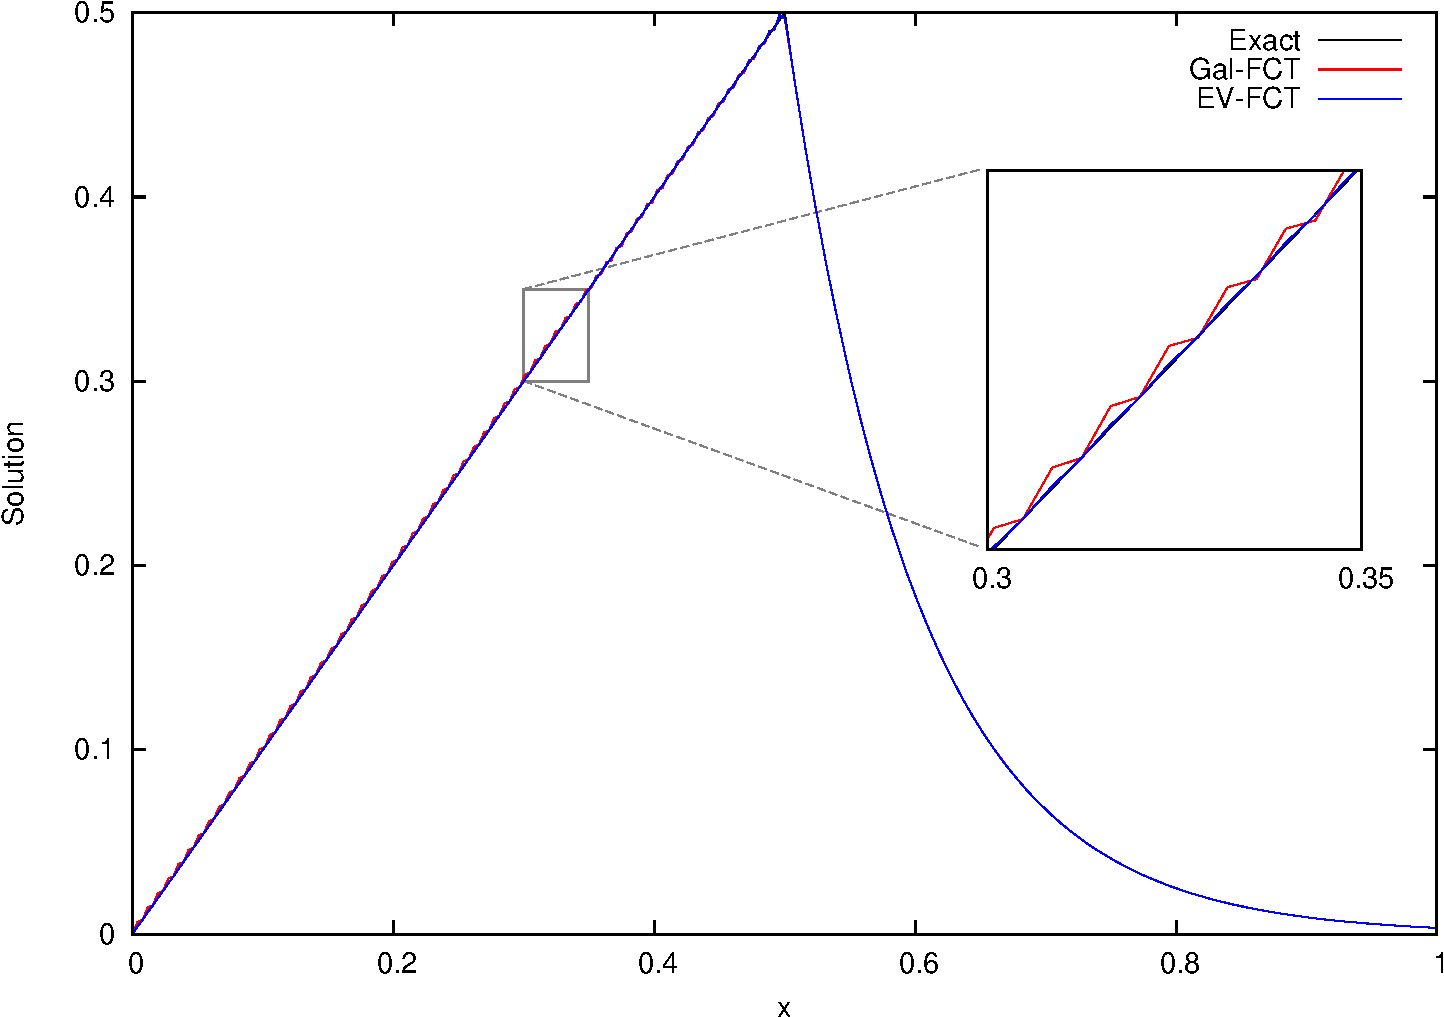
\includegraphics[width=\textwidth]
     {\contentdir/results/transport/source_void_to_absorber/fine.pdf}
   \caption{Comparison of Solutions for Source-Void-to-Absorber Problem
     with $2^8$ Cells}
   \label{fig:source_void_to_absorber_fine}
\end{figure}
%-------------------------------------------------------------------------------

The steady-state results for this test problem revealed some significant
FCT issues regarding the antidiffusion from Dirichlet nodes.
When Dirichlet boundary conditions are strongly imposed, solution
bounds do not apply, and it becomes unclear how to limit antidiffusion
fluxes from these nodes.
Figures \ref{fig:source_void_to_absorber_strong1} and 

%-------------------------------------------------------------------------------
\begin{figure}[ht]
   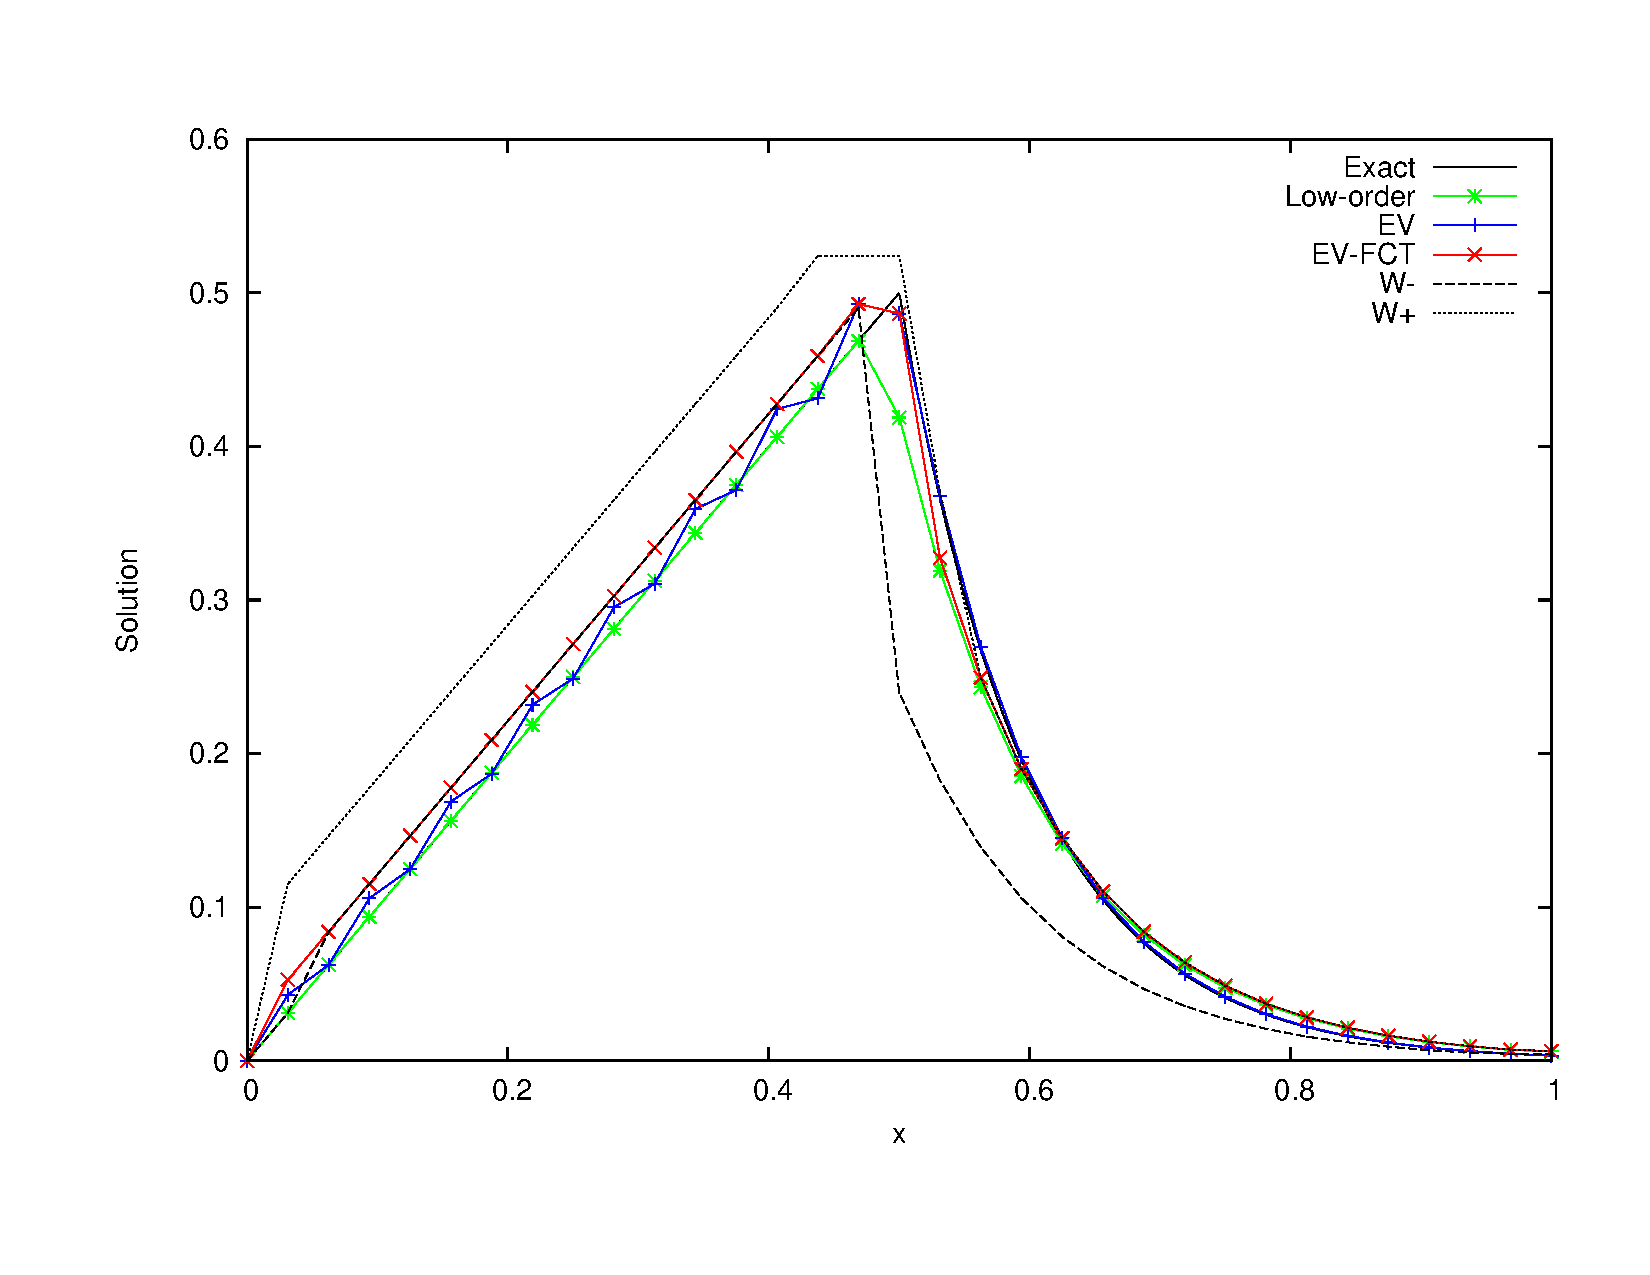
\includegraphics[width=\textwidth]
     {\contentdir/results/transport/source_void_to_absorber/images/strong1.pdf}
   \caption{Solutions for Source-Void-to-Absorber Problem
     with Strongly Imposed Dirichlet Boundary Conditions and $L^-=L^+=1$}
   \label{fig:source_void_to_absorber_strong1}
\end{figure}
%-------------------------------------------------------------------------------
%-------------------------------------------------------------------------------
\begin{figure}[ht]
   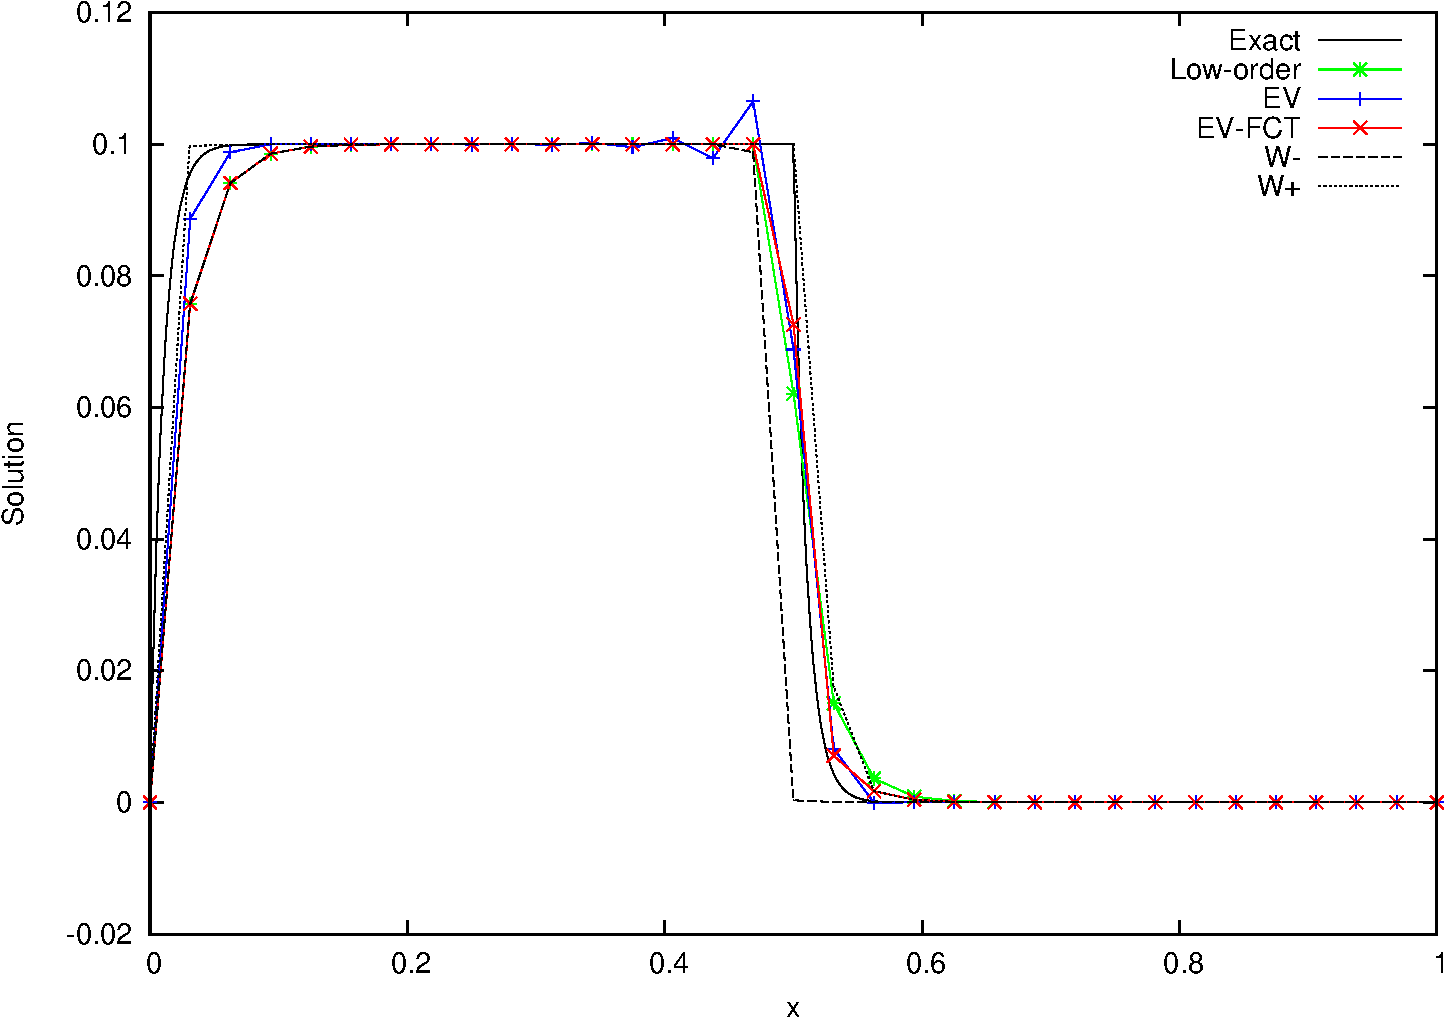
\includegraphics[width=\textwidth]
     {\contentdir/results/transport/source_void_to_absorber/images/strong0.pdf}
   \caption{Solutions for Source-Void-to-Absorber Problem
     with Strongly Imposed Dirichlet Boundary Conditions and $L^-=L^+=0$}
   \label{fig:source_void_to_absorber_strong0}
\end{figure}
%-------------------------------------------------------------------------------
%-------------------------------------------------------------------------------
\begin{figure}[ht]
   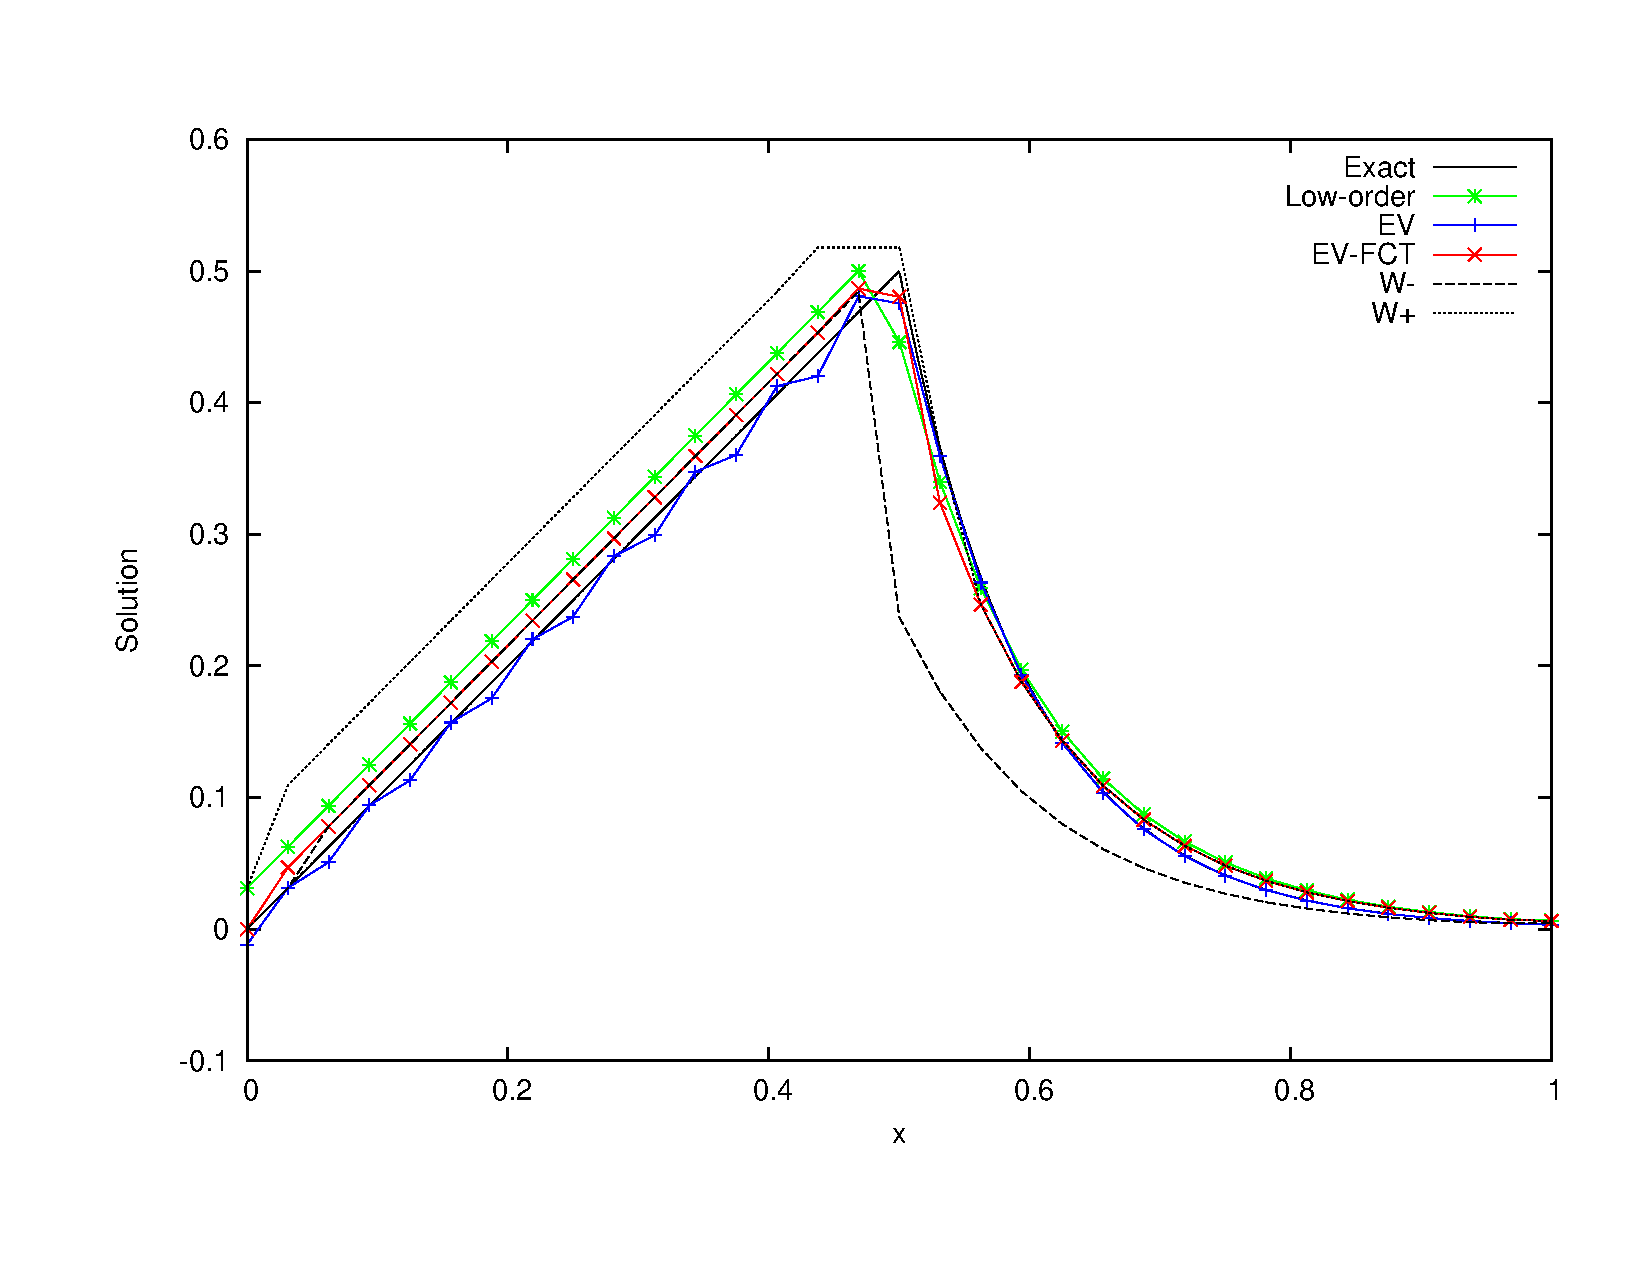
\includegraphics[width=\textwidth]
     {\contentdir/results/transport/source_void_to_absorber/images/weak.pdf}
   \caption{Solutions for Source-Void-to-Absorber Problem
     with Weakly Imposed Dirichlet Boundary Conditions}
   \label{fig:source_void_to_absorber_weak}
\end{figure}
%-------------------------------------------------------------------------------
%-------------------------------------------------------------------------------
\begin{figure}[ht]
   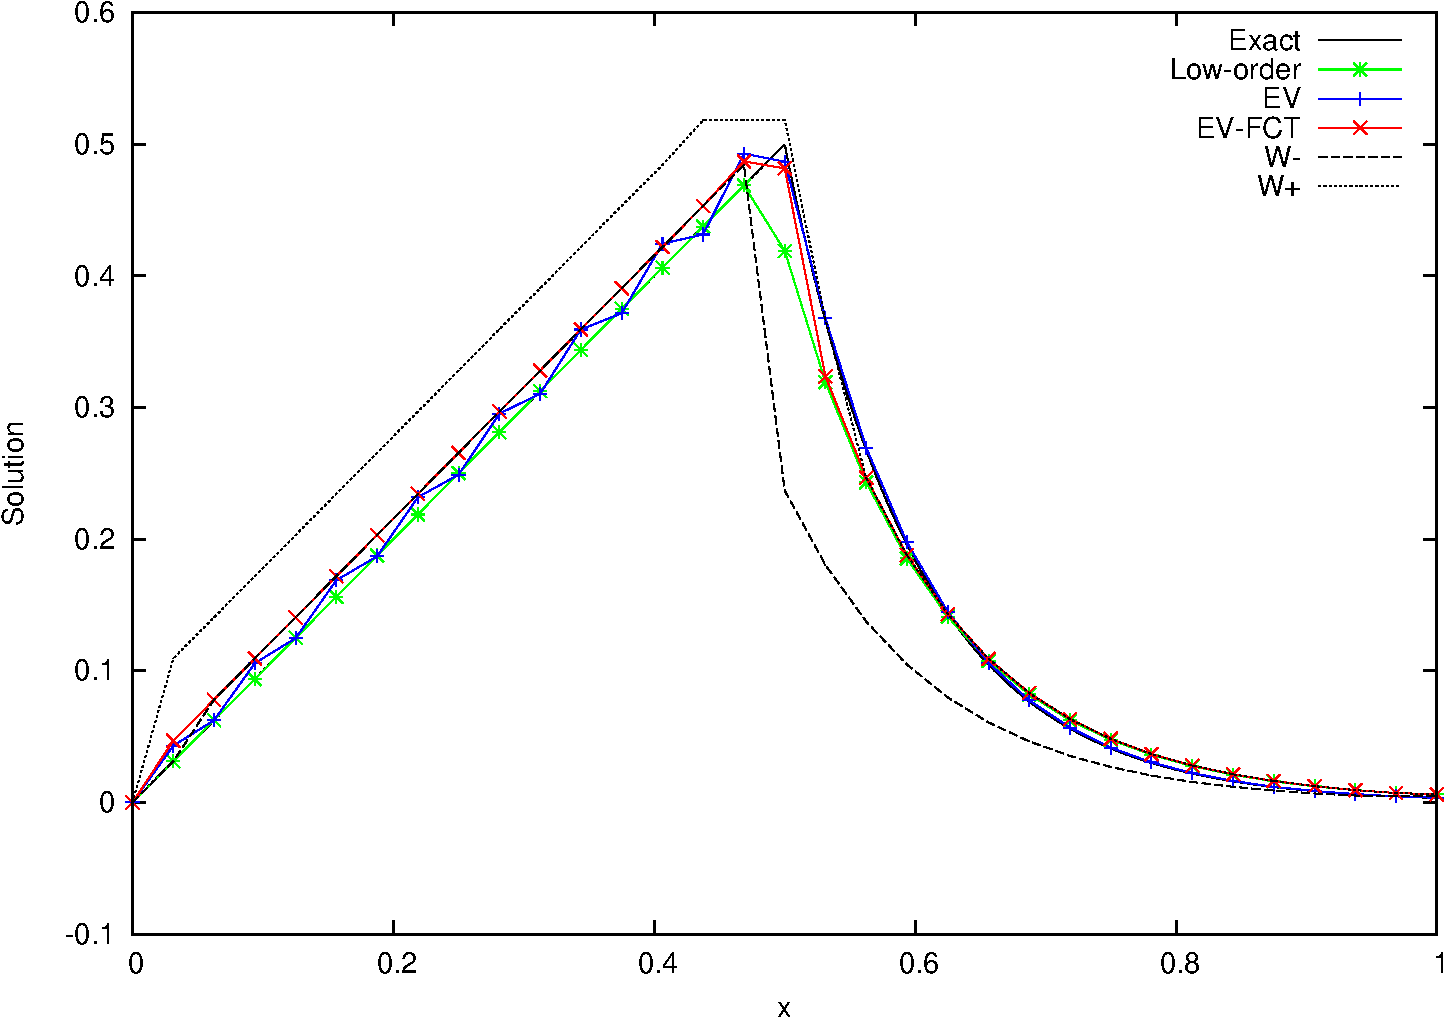
\includegraphics[width=\textwidth]
     {\contentdir/results/transport/source_void_to_absorber/images/weak_with_penalty.pdf}
   \caption{Solutions for Source-Void-to-Absorber Problem
     with Weakly Imposed Dirichlet Boundary Conditions and Boundary Penalty}
   \label{fig:source_void_to_absorber_penalty}
\end{figure}
%-------------------------------------------------------------------------------

\clearpage
